\documentclass[border=10pt]{standalone}
\usepackage{pgfplots}
\pgfplotsset{width=10cm,compat=1.8}
\begin{document}
\begin{tabular}{c}
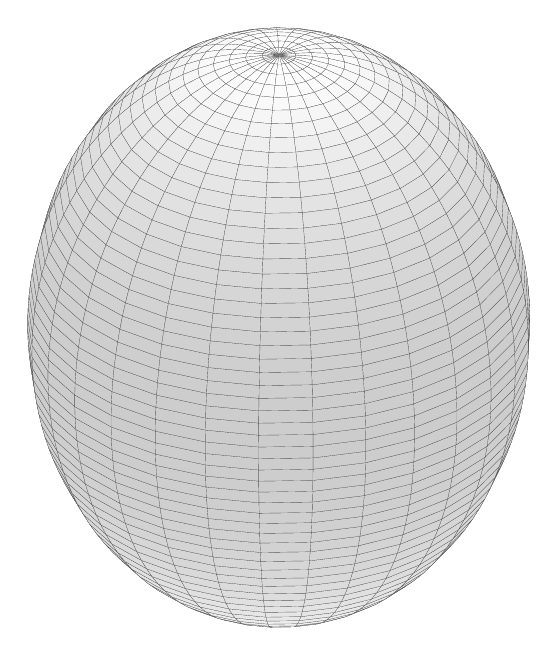
\begin{tikzpicture}
  \begin{axis}[
    hide axis,
    clip=false,
    y domain=0:180,
    samples=30,
    axis equal,
    view={45}{30},
    width=25cm,
    at={(0cm,0cm)},
    %colorbar,
    %colorbar/width=1cm,
    %colorbar horizontal,
    %colorbar style={
    %  height=1cm,
    %  yshift=-0.4cm,
    %  ytick={-1,1}
    %},
    colormap={iron}{[1pt]%
rgb255(-1000pt)=(255,255,255),%
rgb255(-968pt)=(255,255,255),%
rgb255(-936pt)=(254,254,254),%
rgb255(-905pt)=(253,253,253),%
rgb255(-873pt)=(252,252,252),%
rgb255(-841pt)=(250,250,250),%
rgb255(-809pt)=(247,247,247),%
rgb255(-777pt)=(245,245,245),%
rgb255(-745pt)=(242,242,242),%
rgb255(-714pt)=(239,239,239),%
rgb255(-682pt)=(236,236,236),%
rgb255(-650pt)=(232,232,232),%
rgb255(-618pt)=(230,230,230),%
rgb255(-586pt)=(227,227,227),%
rgb255(-554pt)=(224,224,224),%
rgb255(-523pt)=(222,222,222),%
rgb255(-491pt)=(220,220,220),%
rgb255(-459pt)=(218,218,218),%
rgb255(-427pt)=(216,216,216),%
rgb255(-395pt)=(214,214,214),%
rgb255(-363pt)=(213,213,213),%
rgb255(-332pt)=(211,211,211),%
rgb255(-300pt)=(210,210,210),%
rgb255(-268pt)=(209,209,209),%
rgb255(-236pt)=(208,208,208),%
rgb255(-204pt)=(207,207,207),%
rgb255(-172pt)=(206,206,206),%
rgb255(-141pt)=(206,206,206),%
rgb255(-109pt)=(205,205,205),%
rgb255(-77pt)=(205,205,205),%
rgb255(-45pt)=(205,205,205),%
rgb255(-13pt)=(204,204,204),%
rgb255(19pt)=(204,204,204),%
rgb255(50pt)=(205,205,205),%
rgb255(82pt)=(205,205,205),%
rgb255(114pt)=(205,205,205),%
rgb255(146pt)=(206,206,206),%
rgb255(178pt)=(206,206,206),%
rgb255(210pt)=(207,207,207),%
rgb255(241pt)=(208,208,208),%
rgb255(273pt)=(209,209,209),%
rgb255(305pt)=(210,210,210),%
rgb255(337pt)=(211,211,211),%
rgb255(369pt)=(213,213,213),%
rgb255(401pt)=(215,215,215),%
rgb255(432pt)=(216,216,216),%
rgb255(464pt)=(218,218,218),%
rgb255(496pt)=(220,220,220),%
rgb255(528pt)=(222,222,222),%
rgb255(560pt)=(225,225,225),%
rgb255(592pt)=(227,227,227),%
rgb255(623pt)=(230,230,230),%
rgb255(655pt)=(233,233,233),%
rgb255(687pt)=(236,236,236),%
rgb255(719pt)=(239,239,239),%
rgb255(751pt)=(242,242,242),%
rgb255(783pt)=(245,245,245),%
rgb255(814pt)=(248,248,248),%
rgb255(846pt)=(250,250,250),%
rgb255(878pt)=(252,252,252),%
rgb255(910pt)=(253,253,253),%
rgb255(942pt)=(254,254,254),%
rgb255(974pt)=(255,255,255)%
},
    point meta=atan(z/(sqrt(x^2+y^2)))
    ]

  \addplot3 [
      domain=0:360,
      surf,
      shader=flat,
      z buffer=sort,
      %fill=white!50!gray,
      draw=gray!50!black,
      line join=bevel,
      line width=0.002cm,
      samples y=60
    ]
    (
      {(5/sqrt(1+9/16*(1-cos(y)^2)))*sin(y)*cos(x)},
      {(5/sqrt(1+9/16*(1-cos(y)^2)))*sin(y)*sin(x)},
      {(5/sqrt(1+9/16*(1-cos(y)^2)))*cos(y)}
    );
    -- cycle;
   \end{axis}
\end{tikzpicture}
\\
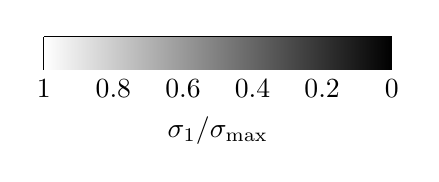
\begin{tikzpicture}
  %A-opt countour
\begin{axis}[%
view={0}{90},
shader=interp,
%3d box=complete,
grid=major,
xlabel = {$\sigma_1/\sigma_{\mathrm{max}}$},
xmin = 0, xmax = 1,
ymin = 0, ymax =1,
view/h=-180,
width=6cm,
height=2cm,
at={(9.5cm,4cm)},
    colormap={blackwhite}{[1cm] rgb255(0cm)=(0,0,0) rgb255(1cm)=(255,255,255)},
yticklabels={,,}
],

\addplot3[%
surf,
samples=30,
domain=0:1,
y domain=0:1,
]
{x};
\end{axis}
\end{tikzpicture}
\end{tabular}
\end{document}